\documentclass[a4paper,12pt]{article}

\usepackage[top = 2.5cm, bottom = 2.5cm, left = 2.5cm, right = 2.5cm]{geometry} 
\usepackage{CJKutf8}
\usepackage[T1]{fontenc}
\usepackage[utf8]{inputenc}
\usepackage{multirow} 
\usepackage{booktabs}
\usepackage{longtable}
\usepackage{enumitem}
\setitemize{noitemsep,topsep=0pt,parsep=0pt,partopsep=0pt}
\renewcommand{\labelitemi}{$\diamond$}
\usepackage{listings}
\usepackage[table]{xcolor}
\usepackage{graphicx}
\usepackage{caption}
\usepackage{setspace}
\setlength{\parindent}{0in}
\usepackage{float}
\usepackage{fancyhdr}
\pagestyle{fancy}
\fancyhf{}
\setlength{\headheight}{16pt}
\newcommand{\selfjp}{\begin{CJK*}{UTF8}{min}ドゥーマ\end{CJK*}}
\newcommand{\source}[1]{\caption*{Source: {#1}} }
\newcommand{\htmlelem}[1]{\lstinline[columns=fixed,language=HTML]{#1}}
\newcommand{\nsp}{\vspace{0.05cm}\\}
\lhead{\footnotesize Web Development: Lesson 2}
\rhead{\footnotesize Doomer / \selfjp}
\cfoot{\footnotesize \thepage} 

\definecolor{codegreen}{rgb}{0,0.6,0}
\definecolor{codegray}{rgb}{0.5,0.5,0.5}
\definecolor{codepurple}{rgb}{0.58,0,0.82}
\definecolor{backcolour}{rgb}{0.95,0.95,0.92}
\lstdefinestyle{mystyle}{
    backgroundcolor=\color{backcolour},   
    commentstyle=\color{codegreen},
    keywordstyle=\color{magenta},
    numberstyle=\tiny\color{codegray},
    stringstyle=\color{codepurple},
    basicstyle=\ttfamily\footnotesize,
    breakatwhitespace=false,         
    breaklines=true,                 
    captionpos=b,                    
    keepspaces=true,                 
    numbers=left,                    
    numbersep=5pt,                  
    showspaces=false,                
    showstringspaces=false,
    showtabs=false,                  
    tabsize=2
}
\lstset{style=mystyle}

\begin{document}

\thispagestyle{empty} 

\begin{tabular}{p{15.5cm}} 
{\large \bf Web Development: Lesson 2} \\
Discord Lessons\\ Fall 2020\\ Doomer / \selfjp \\
\hline
\\
\end{tabular}

\vspace*{0.3cm}

\begin{center}
	{\Large \bf Lesson 2 - Cascading Style Sheets}
	\vspace{2mm}\\
	{\bf dedicated to Spennorex and Grumpah}
		
\end{center}  

\vspace{0.4cm}

\section{Introduction}
This time we'll work on the design and styling of our web page. Style is important, because it makes pages look beautiful and sometimes helps to find features easier, due to certain conventions, choice of color, etc. 

\section{CSS Structure}
A basic CSS document, would look like this:

\begin{lstlisting}[caption=Sample CSS Script,label={lst:sample_1}]
body {
    background-color: dodgerblue;
    color: #DC143C;
}
\end{lstlisting}
This basic style sheet, would cause the \htmlelem{<body>} to have a dodgerblue background color and a crimson font color. There are a few pre-defined colors, which I'll show you later and you can pick any custom color using the hexadecimal color codes, which you can get from most color pickers. There are a lot more CSS Properties, so let's dive right into it.

\section{CSS Properties}
'background-color' or 'color' are called \textbf{CSS properties}. I'll give you a list of these properties with examples - most of these properties are pretty intuitive. As for the background we have multiple CSS properties:
\begin{itemize}
    \item background-color: chocolate;
    \item background-image: url"(./img/test.png");
    \item opacity: 0.5;
    \item color: cornsilk;
    \item font: 20px Arial, sans-serif;
    \item font-weight: bold;
    \item display: block;
    \item margin: 10px;
    \item padding: 10px;
    \item border: 10px solid black;
    \item border-radius: 4px;
\end{itemize}
The margin, padding, border and border radius properties can be explained using the css box-model:\\
\begin{figure}[h!]
    \centering
    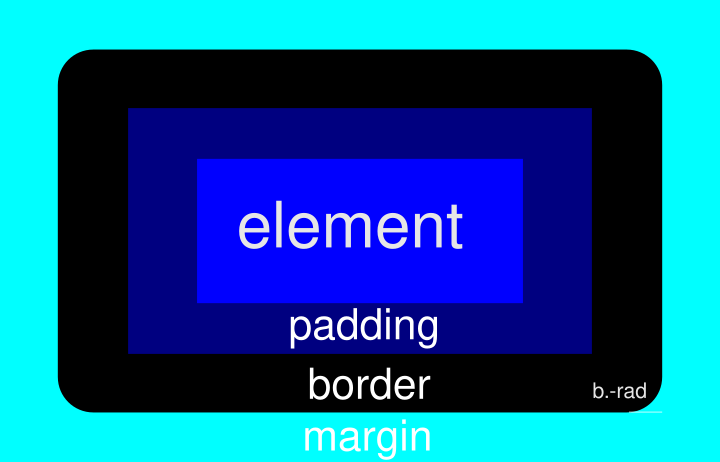
\includegraphics[width=0.5\textwidth]{imgs/css-box-model}
    \caption{CSS Box Model}
    \label{fig:css-box-model}
\end{figure}

The element is the whole element with its contents, such as in the case of \htmlelem{<p>Text</p>}: "Text". The element can have a border, and you can set the space between the element and the border using the padding property. To adjust the spacing between two elements you can increase the margin. There are different units for measuring distance, which we'll cover soon.\nsp
There are also background properties, such as the 'background-color' and the 'background-image'. These allow you to give an element a certain background-color or in the case of body, you can give the whole page a background-color or image, also the opacity property allows to control the alpha-channel of the background, while the color allows you to pick a font-color, to use on the element.\nsp
Another very important property is the 'display' property, which defines how the element is displayed (in context of other elements). There are following values for the display property:
\begin{itemize}
    \item none
    \item inline
    \item block
    \item inline-block
\end{itemize}
The 'none' is pretty intuitive: it doesn't show the element at all, 'inline' means, that the element just get's packed with the neighbour elements in one line. 'block' means that we pack the element into below the previous element and give the element width and height properties, which can be changed to increase / decrease the element box. Same goes for 'inline-block' except for not being placed below, but next to the previous element.

\section{CSS Units}
Here you have a small (distance) unit reference:\\
Let's start off with the Absolute Lengths:\\
\begin{tabular}{|c|c|}
    \hline
    cm & Centimeters                \\
    mm & Millimeters                \\
    in & Inches                     \\
    px & Pixels (1/96th of an Inch) \\
    pt & Points (1/72th of an Inch) \\
    pc & Picas  (1/6th of an Inch)  \\
    \hline
\end{tabular}\nsp\nsp
And follow up with the relative ones:\\
\begin{tabular}{|c|c|}
    \hline
    em & Relative to the font-size of the element       \\
    ex & Relative to the x-height of the current font   \\
    ch & Relative to the width of the "0" (a character) \\
    rem & Relative to font-size of the root element     \\
    vw & Relative to 1\% of the width of the viewport*  \\
    vh & Relative to 1\% of the height of the viewport* \\
    \% &  	Relative to the parent element              \\
    \hline
\end{tabular}

\section{CSS Colors}
Now let's cover the different predefined CSS colors. Here you'll have a colorpalette of those:\\
\begin{center}
\setlength{\arrayrulewidth}{1mm}
\setlength{\tabcolsep}{18pt}
\arrayrulecolor[HTML]{FFFFFF}
\begin{longtable}{|p{0.25\textwidth}|p{0.28\textwidth}|p{0.22\textwidth}|}
    \hline
    \cellcolor[HTML]{F0F8FF} AliceBlue         & \cellcolor[HTML]{FAEBD7} AntiqueWhite         & \cellcolor[HTML]{00FFFF} Aqua            \\ \hline
    \cellcolor[HTML]{FFE4C4} Bisque            & \cellcolor[HTML]{000000} Black                & \cellcolor[HTML]{FFEBCD} BlanchedAlmond  \\ \hline
    \cellcolor[HTML]{0000FF} Blue              & \cellcolor[HTML]{8A2BE2} BlueViolet           & \cellcolor[HTML]{A52A2A} Brown           \\ \hline
    \cellcolor[HTML]{DEB887} BurlyWood         & \cellcolor[HTML]{5F9EA0} CadetBlue            & \cellcolor[HTML]{7FFF00} Chartreuse      \\ \hline
    \cellcolor[HTML]{D2691E} Chocolate         & \cellcolor[HTML]{FF7F50} Coral                & \cellcolor[HTML]{6495ED} CornflowerBlue  \\ \hline
    \cellcolor[HTML]{FFF8DC} Cornsilk          & \cellcolor[HTML]{DC143C} Crimson              & \cellcolor[HTML]{00FFFF} Cyan            \\ \hline
    \cellcolor[HTML]{00008B} DarkBlue          & \cellcolor[HTML]{008B8B} DarkCyan             & \cellcolor[HTML]{B8860B} DarkGoldenRod   \\ \hline
    \cellcolor[HTML]{A9A9A9} DarkGray          & \cellcolor[HTML]{A9A9A9} DarkGrey             & \cellcolor[HTML]{006400} DarkGreen       \\ \hline
    \cellcolor[HTML]{BDB76B} DarkKhaki         & \cellcolor[HTML]{8B008B} DarkMagenta          & \cellcolor[HTML]{556B2F} DarkOliveGreen  \\ \hline
    \cellcolor[HTML]{FF8C00} DarkOrange        & \cellcolor[HTML]{9932CC} DarkOrchid           & \cellcolor[HTML]{8B0000} DarkRed         \\ \hline
    \cellcolor[HTML]{E9967A} DarkSalmon        & \cellcolor[HTML]{8FBC8F} DarkSeaGreen         & \cellcolor[HTML]{483D8B} DarkSlateBlue   \\ \hline
    \cellcolor[HTML]{2F4F4F} DarkSlateGray     & \cellcolor[HTML]{2F4F4F} DarkSlateGrey        & \cellcolor[HTML]{00CED1} DarkTurquoise   \\ \hline
    \cellcolor[HTML]{9400D3} DarkViolet        & \cellcolor[HTML]{FF1493} DeepPink             & \cellcolor[HTML]{00BFFF} DeepSkyBlue     \\ \hline
    \cellcolor[HTML]{696969} DimGray           & \cellcolor[HTML]{696969} DimGrey              & \cellcolor[HTML]{1E90FF} DodgerBlue      \\ \hline
    \cellcolor[HTML]{B22222} FireBrick         & \cellcolor[HTML]{FFFAF0} FloralWhite          & \cellcolor[HTML]{228B22} ForestGreen     \\ \hline
    \cellcolor[HTML]{FF00FF} Fuchsia           & \cellcolor[HTML]{DCDCDC} Gainsboro            & \cellcolor[HTML]{F8F8F8} GhostWhite      \\ \hline
    \cellcolor[HTML]{FFD700} Gold              & \cellcolor[HTML]{DAA520} GoldenRod            & \cellcolor[HTML]{808080} Gray            \\ \hline
    \cellcolor[HTML]{808080} Grey              & \cellcolor[HTML]{008000} Green                & \cellcolor[HTML]{ADFF2F} GreenYellow     \\ \hline
    \cellcolor[HTML]{F0FFF0} HoneyDew          & \cellcolor[HTML]{FF69B4} HotPink              & \cellcolor[HTML]{CD5C5C} IndianRed       \\ \hline
    \cellcolor[HTML]{4B0082} Indigo            & \cellcolor[HTML]{FFFFF0} Ivory                & \cellcolor[HTML]{F0E68C} Khaki           \\ \hline
    \cellcolor[HTML]{E6E6FA} Lavender          & \cellcolor[HTML]{FFF0F5} LavenderBlush        & \cellcolor[HTML]{7CFC00} LawnGreen       \\ \hline
    \cellcolor[HTML]{FFFACD} LemonChiffon      & \cellcolor[HTML]{ADD8E6} LightBlue            & \cellcolor[HTML]{F08080} LightCoral      \\ \hline
    \cellcolor[HTML]{E0FFFF} LightCyan         & \cellcolor[HTML]{FAFAD2} LightGoldenRodYellow & \cellcolor[HTML]{D3D3D3} LightGray       \\ \hline
    \cellcolor[HTML]{D3D3D3} LightGrey         & \cellcolor[HTML]{90EE90} LightGreen           & \cellcolor[HTML]{FFB6C1} LightPink       \\ \hline
    \cellcolor[HTML]{FFA07A} LightSalmon       & \cellcolor[HTML]{20B2AA} LightSeaGreen        & \cellcolor[HTML]{87CEFA} LightSkyBlue    \\ \hline
    \cellcolor[HTML]{778899} LightSlateGray    & \cellcolor[HTML]{778899} LightSlateGrey       & \cellcolor[HTML]{B0C4DE} LightSteelBlue  \\ \hline
    \cellcolor[HTML]{FFFFE0} LightYellow       & \cellcolor[HTML]{00FF00} Lime                 & \cellcolor[HTML]{32CD32} LimeGreen       \\ \hline
    \cellcolor[HTML]{FAF0E6} Linen             & \cellcolor[HTML]{FF00FF} Magenta              & \cellcolor[HTML]{800000} Maroon          \\ \hline
    \cellcolor[HTML]{66CDAA} MediumAquaMarine  & \cellcolor[HTML]{0000CD} MediumBlue           & \cellcolor[HTML]{CA55D3} MediumOrchid    \\ \hline
    \cellcolor[HTML]{9370DB} MediumPurple      & \cellcolor[HTML]{3CB371} MediumSeaGreen       & \cellcolor[HTML]{7B68EE} MediumSlateBlue \\ \hline
    \cellcolor[HTML]{00FA9A} MediumSpringGreen & \cellcolor[HTML]{48D1CC} MediumTurquoise      & \cellcolor[HTML]{C71585} MediumVioletRed \\ \hline
    \cellcolor[HTML]{191970} MidnightBlue      & \cellcolor[HTML]{F5FFFA} MintCream            & \cellcolor[HTML]{FFE4E1} MistyRose       \\ \hline
    \cellcolor[HTML]{FFE4B5} Moccasin          & \cellcolor[HTML]{FFDEAD} NavajoWhite          & \cellcolor[HTML]{000080} Navy            \\ \hline
    \cellcolor[HTML]{FDF5E6} OldLace           & \cellcolor[HTML]{808000} Olive                & \cellcolor[HTML]{6B8E23} OliveDrab       \\ \hline
    \cellcolor[HTML]{FFA500} Orange            & \cellcolor[HTML]{FF4500} OrangeRed            & \cellcolor[HTML]{DA70D6} Orchid          \\ \hline
    \cellcolor[HTML]{EEE8AA} PaleGoldenRod     & \cellcolor[HTML]{98FB98} PaleGreen            & \cellcolor[HTML]{AFEEEE} PaleTurquoise   \\ \hline
    \cellcolor[HTML]{DB7093} PaleVioletRed     & \cellcolor[HTML]{FFEFD5} PapayaWhip           & \cellcolor[HTML]{FFDAB9} PeachPuff       \\ \hline
    \cellcolor[HTML]{CD853F} Peru              & \cellcolor[HTML]{FFC0CB} Pink                 & \cellcolor[HTML]{DDA0DD} Plum            \\ \hline
    \cellcolor[HTML]{B0E0E6} PowderBlue        & \cellcolor[HTML]{800080} Purple               & \cellcolor[HTML]{663399} RebeccaPurple   \\ \hline
    \cellcolor[HTML]{FF0000} Red               & \cellcolor[HTML]{BC8F8F} RosyBrown            & \cellcolor[HTML]{4169E1} RoyalBlue       \\ \hline
    \cellcolor[HTML]{8B4513} SaddleBrown       & \cellcolor[HTML]{FA8072} Salmon               & \cellcolor[HTML]{F4A460} SandyBrown      \\ \hline
    \cellcolor[HTML]{2E8B57} SeaGreen          & \cellcolor[HTML]{FFF5EE} SeaShell             & \cellcolor[HTML]{A0522D} Sienna          \\ \hline
    \cellcolor[HTML]{C0C0C0} Silver            & \cellcolor[HTML]{87CEEB} SkyBlue              & \cellcolor[HTML]{6A5ACD} SlateBlue       \\ \hline
    \cellcolor[HTML]{708090} SlateGray         & \cellcolor[HTML]{708090} SlateGrey            & \cellcolor[HTML]{FFFAFA} Snow            \\ \hline
    \cellcolor[HTML]{00FF7F} SpringGreen       & \cellcolor[HTML]{4682B4} SteelBlue            & \cellcolor[HTML]{D2B48C} Tan             \\ \hline
    \cellcolor[HTML]{008080} Teal              & \cellcolor[HTML]{D8BFD8} Thistle              & \cellcolor[HTML]{FF6347} Tomato          \\ \hline
    \cellcolor[HTML]{40E0D0} Turquoise         & \cellcolor[HTML]{EE82EE} Violet               & \cellcolor[HTML]{F5DEB3} Wheat           \\ \hline
    \cellcolor[HTML]{FFFFFF} White             & \cellcolor[HTML]{F5F5F5} WhiteSmoke           & \cellcolor[HTML]{FFFF00} Yellow          \\ \hline
\end{longtable}
\end{center}
\newpage

\section{CSS Selectors}
At last before implementing our stylesheet into our web page, we need to discuss how to assign our \textbf{CSS Rules} to the correct elements:\nsp
If you're referring to a ..., you need to use... \nsp
\setlength{\arrayrulewidth}{0.4pt}
\setlength{\tabcolsep}{6pt}
\arrayrulecolor[HTML]{000000}
\begin{tabular}{|l|c|}
    \hline
    element e & \htmlelem{e \{\}} \\
    class c & \htmlelem{.c \{\}} \\
    id i & \htmlelem{#i \{\}} \\
    element e with class c & \htmlelem{e.c \{\}} \\
    element e inside element a & \htmlelem{a e \{\}} \\
    element attribute a & \htmlelem{[a] \{\}}\\
    \hline
\end{tabular}\nsp
There are a few more things, but you'll see them live in action in the next Listing :).


\section{Implementing into our Web Page}
\begin{lstlisting}[language=HTML,caption=Updated Wireframe,label={lst:html_wireframe}]
<html>
    <head>
        <title></title>
        <style>
        </style>
    </head>
    <body>
    </body>
</html>
\end{lstlisting}
\newpage
Now let's decorate our previous site, with a bit of css.
\begin{lstlisting}[language=HTML,caption=Content Update,label={lst:styled_html}]
<html>
    <head>
        <title>My Profile</title>
        <style>
        body {
            background-image: url(https://external-content.duckduckgo.com/iu/?u=http%3A%2F%2Fwallsdesk.com%2Fwp-content%2Fuploads%2F2016%2F05%2FSakura-images.jpg&f=1&nofb=1);
            background-size: cover;
            background-position: center;
            background-repeat: no-repeat;
            height: 100%; 
        }
        .text {
	        background-color: rgb(0,0,0);
	        background-color: rgba(0,0,0, 0.65);
	        color: powderblue;
	        font-weight: bold;
	        border: 3px solid #f1f1f1;
	        position: absolute;
	        top: 30vh;
	        left: 30vw;
	        width: 40vw;
	        padding: 20px;
        }
        </style>
    </head>
    <body>
        <div class="text">
            <h1>My Profile Page</h1>
            <p>Here's who I am :)</p>
            <ol>
            	<li>Name: Doomer</li>
            	<li>How many Discord Notifications do you have? 0</li>
            	<li>Gender: genderfluid</li>
            	<li>Birthday: 22nd of December</li>
            	<li>Timezone: UTC+2 (CET)</li>
            	<li>Languages Spoken: English, Russian, German</li>
            	<li>Favorite Colors: Black, Blue, Purple</li>
            	<li>...</li>
            </ol>
            <p>I think that's enough <br/> for an example.</p>
        </div>
    </body>
</html>
\end{lstlisting}

\newpage
\section{Excercises}
These excercises are optional and you can do them if you want to get experience and feel comfortable using the style sheets:
\begin{enumerate}
    \item Try to interpret unknown elements, attributes and and understand the parts of Listing \ref{lst:styled_html}.
    \item Style the pages from Lesson 1. Go wild!
\end{enumerate}

\section{Final Notes}
Thanks a lot for reading this lesson! Hope it tought you something. As always, if you have questions, drop them in Discord (Doomer\#1718). I think this was a rather large script, with a lot of theory, maybe that's because of the color table, maybe, because of the last listing - I don't know, but I'm satisfied. If you have any suggestions on how to improve the script, e.g. if I forgot something, made a typo somewhere or left out an important concept. If you want to show me your page or want to have tips regarding it, simply ask and would be good if you'd provide the affected code snippets. See ya in the next one, I guess.

\end{document}
